% !TEX encoding = IsoLatin

% La riga soprastante serve per configurare gli editor TeXShop, TeXWorks
% e TeXstudio per gestire questo file con la codifica IsoLatin o Latin 1
% o ISO 8859-1.

% per commentare una riga mettere % al suo inizio
% per s-commentare una riga (ossia attivarla) togliere il % al suo inizio
%


\documentclass[%pdfa% formato PDF/A, obbligatorio per l'archiviazione delle tesi di Polito
  cucitura%lascia margine per la rilegatura
  %,twoside% per stampa fronte-retro (fortemente consigliato per tesi voluminose, opzionale per le altre)
  ,english
  ,12pt% font più grande (12pt) rispetto a quello normalmente usato (11pt)
  ,openright
  ]{toptesi}


\usepackage{hyperref}
\hypersetup{%
    pdfpagemode={UseOutlines},
    bookmarksopen,
    pdfstartview={FitH},
    colorlinks,
    linkcolor={blue},
    citecolor={red},
    urlcolor={blue}
  }
% \documentclass[11pt,twoside,oldstyle,autoretitolo,classica,greek]{toptesi}
% \usepackage[or]{teubner}
%%%%%%%%%%%%%%%%%%%%%%%%%%%%%%%%%%%%%%%%%%%%%%%%%%%%
%
% Esempio di composizione di tesi di laurea.
%
% Questo esempio e' stato preparato inizialmente 13-marzo-1989
% e poi e' stato modificato via via che TOPtesi andava
% arricchendosi di altre possibilita'.
%
% Nel seguito laurea "quinquennale" sta anche per "specialistica" o "magistrale"

% Cambiare encoding a piacere; oppure non caricare nessun encoding se si usano
% solo caratteri a 7 bit (ASCII) nei file d'entrata.
%
\usepackage[latin1]{inputenc}% IMPORTANTE! usare codifica ISO-8859-1 per le lettere accentate


% !TEX encoding = IsoLatin

% per inserire uno spazio "fantasma" nella definizione di un'abbreviazione
\usepackage{xspace}

% per inserire un DOI senza problemi coi caratteri "strani" ivi presenti
\usepackage{doi}
\renewcommand{\doitext}{DOI }% originally was "doi:"

% per inserire correttamente le unit� di misura SI (incluse quelle binarie)
\usepackage[binary-units]{siunitx}
% se si desidera usare / invece che la potenza -1 per indicare "al secondo"
\sisetup{per-mode=symbol}

% per inserire codice di programmazione complesso
\usepackage{listings}% per inserire codice di programmazione complesso
\lstset{
basicstyle=\ttfamily,
columns=fullflexible,
xleftmargin=3ex,
breaklines,
breakatwhitespace,
escapechar=`
}

% modify some page parameters
\setlength{\parskip}{\medskipamount}

% riga orizzontale
\newcommand{\HRule}{\rule{\linewidth}{0.2mm}}
% esempio di creazione di semplici abbreviazioni
\newcommand{\ltx}{\LaTeX\xspace}
\newcommand{\txw}{TeXworks\xspace}
\newcommand{\mik}{MikTex\xspace}
\newcommand{\html}{HTML\xspace}
\newcommand{\xhtml}{XHTML\xspace}

% esempio di creazione di un'abbreviazione con un parametro (il cui uso � indicato da #1)
\newcommand{\cmd}[1]{\texttt{#1}\xspace}
% per citare un RFC, es. \rfc{822}
\newcommand{\rfc}[1]{RFC-#1\xspace}
% per citare un file (es. \file{autoexec.bat}) o una URI fittizia (es. \file{http://www.lioy.it/})
% per le URI vere usare \url o \href
\newcommand{\file}[1]{\texttt{#1}\xspace}
% per inserire codice di esempio in-line
\newcommand{\code}[1]{\lstinline|#1|}
% importante per i pathname Windows perch� non si pu� usare \ essendo un carattere riservato di Latex
\newcommand{\bs}{\textbackslash}
% definizione di un termine: formattazione ed inserimento nell'indice
\newcommand{\tdef}[1]{\textit{#1}\index{#1}}
% meta-termine, usato tipicamente nelle definizioni dei tag
\newcommand{\meta}[1]{\textit{#1}}
% abbreviazioni in inglese
\newcommand{\ie}{i.e.\xspace}
\newcommand{\eg}{e.g.\xspace}



%%% TODO: XXX My commands XXX
% Shortcuts 
\newcommand{\bt}[1]{\textbf{#1}}  %%bold text
\newcommand{\ita}[1]{\textit{#1}}  %%italic text
\newcommand{\bit}[1]{\textbf{\textit{#1}}} %%bold italic
\newcommand{\q}[1]{``#1''} %%bold italic
\newcommand{\plchld}[1]{\bt{\color{red}This chapter/section has to be write yet.}} %%placeholder
% Recurrent terms
\newcommand{\krack}{KRACK\xspace}
\newcommand{\fwh}{4-Way Handshake\xspace}

%Placeholder for images
\newcommand{\dummyfig}[1]{
  \centering
  \fbox{
    \begin{minipage}[c][0.33\textheight][c]{0.5\textwidth}
      \centering{#1}
    \end{minipage}
  }
}


\selectlanguage{english}



\begin{document}

\english

\ateneo{Politecnico di Torino}

%%% scegliere la propria facolt� (solo PRIMA dell'AA 2012-2013)
%
%\facolta[III]{Ingegneria dell'Informazione}
%\facolta[IV]{Organizzazione d'Impresa\\e Ingegneria Gestionale}
%\Materia{Remote sensing}% uso sconsigliato

%\monografia{Gestione informatizzata di un magazzino ricambi}% per la laurea triennale
\titolo{Security Analysis of the WPA2 KRACK patches}% per la laurea quinquennale e il dottorato
%\sottotitolo{Metodo dei satelliti medicei}% NON obbligatorio, per la laurea quinquennale e il dottorato
\CorsoDiLaureaIn{Master Degree in }

%%% scegliere il proprio corso
%
%\corsodilaurea{Ingegneria dell'Organizzazione d'Impresa}% per la laurea di primo e secondo livello
%\corsodilaurea{Ingegneria Logistica e della Produzione}% per la laurea di primo e secondo livello
%\corsodilaurea{Ingegneria Gestionale}% per la laurea di primo e secondo livello
\corsodilaurea{Computer Engineering}% per la laurea di primo e secondo livello
%\corsodidottorato{Meccanica}% per il dottorato

\TesiDiLaurea{Master Thesis}

\CandidateName{Candidate}
\candidato{Graziano \textsc{Marallo}}% per tutti i percorsi
%\secondocandidato{Evangelista \textsc{Torricelli}}% per la laurea magistrale solamente
%\direttore{prof. Albert Einstein}% per il dottorato
%\coordinatore{prof. Albert Einstein}% per il dottorato
\AdvisorName{Supervisors}
\relatore{prof.\ Antonio Lioy}% per la laurea e il dottorato
\secondorelatore{prof.\ Jan Tobias Muehlberg}
%\secondorelatore{dipl.~ing.~Werner von Braun}% per la laurea magistrale
%\terzorelatore{{\tabular{@{}l}dott.\ Neil Armstrong\\prof. Maria Rossi\endtabular}}% per la laurea magistrale
%\tutore{ing.~Karl Von Braun}% per il dottorato
%\tutoreaziendale{dott.\ ing.\ Giovanni Giacosa} % solo per la laurea di secondo livello con tesi svolta in azienda
%\NomeTutoreAziendale{Supervisore aziendale\\Centro Ricerche FIAT}
%\sedutadilaurea{Agosto 1615}% per la laurea quinquennale
%\esamedidottorato{Novembre 1610}% per il dottorato
%\sedutadilaurea{\textsc{Novembre} 2017}% per la laurea triennale
\sedutadilaurea{\textsc{Academic~year} 2018-2019}% per la laurea magistrale
%\annoaccademico{1615-1616}% solo con l'opzione classica
%\annoaccademico{2006-2007}% idem
%\ciclodidottorato{XV}% per il dottorato
\logosede{images/logopolito}
%
%\chapterbib %solo per vedere che cosa succede; e' preferibile comporre una sola bibliografia
%\AdvisorName{Supervisors}
%\newtheorem{osservazione}{Osservazione}% Standard LaTeX

%\usepackage[a-1b]{pdfx}
%\hypersetup{%
%    pdfpagemode={UseOutlines},
%    bookmarksopen,
%    pdfstartview={FitH},
%    colorlinks,
%    linkcolor={blue},
%    citecolor={green},
%    urlcolor={blue}
%  }

%
% per numerare e far comparire nell'indice anche le sezioni di quarto livello
% SCONSIGLIATO! da usarsi solo in caso di estrema necessit�
%\setcounter{secnumdepth}{4}% section-numbering-depth
%\setcounter{tocdepth}{4}% TOC-numbering-depth (TOC=Table-Of-Content)

%\setbindingcorrection{3mm}

\errorcontextlines=9

\frontespizio
\paginavuota
\newpage
%per sfruttare meglio lo spazio nella pagina
\advance\voffset -5mm
\advance\textheight 30mm

% opzionale, solo se si vuole dedicare la tesi a delle persone care
\begin{dedica}
A mio padre

\textdagger\ A mio nonno Pino
\end{dedica}

\sommario
TODO

\ringraziamenti

TODO

%% inserire sempre nella tesi per la laurea di I livello, perch� il nome dei tutori non � indicato sul frontespizio.
%Il lavoro descritto in questa monografia � stato svolto sotto la supervisione
%del Prof. Antonio Lioy (tutore accademico)% inserire sempre il nome del tutore accademico
% e dell'Ing. Mario Rossi (tutore aziendale)% inserire solo se la monografia � relativa ad un tirocinio.
%.

%\tablespagetrue % normalmente questa riga non serve ed e' commentata
%\figurespagetrue % normalmente questa riga non serve ed e' commentata

\indici

\mainmatter

\chapter{Introduction}

% !TEX encoding = IsoLatin


Vulnerabilities, in the last few years, have become on the main cause of threats in cyberspace security. 
A vulnerability is basically, as defined in RFC 2828, a flaw or weakness in a system's design, implementation, 
or operation and management that could be exploited to violate the system's security policy. 
Since they are so important and meaningful, a lots of work has been done in order to fight and in a certain way stem the attacks. 
Various technique can be used like static  analysis, dynamic, symbolic execution and fuzzing.
Our main interest is on the fuzzing one. Fuzzing, basically, requires less knowledge of the target, 
and for this reason can be easily adapted and scaled to a large variety of situation and problem. 
Due to this reason is the de facto the most popular vulnerability discovery solution.


\section{Fuzzing} %%UPDATE

\subsection{General background}

Attack on vulnerabilities, especially the ones made for example on zero day vulnerability, are seriously dangerous and sometime can brought to critical situation as well.
So much of the effort of the research carry out nowadays is done on vulnerability discovery techniques towards software and information system. One of the main technique on 
which the attention has been focused on without any doubt, is fuzzing. But is fuzzing and how it works? 

The concept of fuzzing was initially proposed in the 1990's, and even though the concept has remained unchanged,
the way of how fuzzing can be done has grown exponentially and evolved as well in the last few years. On the other hand, through the years has been noticed that fuzzing tends to
to find simple memory corruption bugs and cover a small part of the the target code provided, and so as a result a low efficiency in findings major or critical flaws.
Using a combination of feedback-driven fuzzing mode and genetic algorithms can provide a more flexible and customizable fuzzing framework that  makes the fuzzing process more clever and in a certain way more efficient as well.


\subsection{Fuzzing process}

Fuzzing is basically the most popular vulnerability discovery technique used today.
It stars with generating massive normal and abnormal inputs towards application and at the same time try to detect exception by feeding generated inputs to the target applications and carefully monitoring each execution states.
In comparison with other techniques, fuzzing present itself as easier in deploying and plus it allows to perform analysis even without the source code. Another remarkable feature is that fuzzing tests is performed during real execution
and for this reason it gains an higher accuracy; moreover it requires a very small knowledge of the target application, resulting a scalability gain. 
Nevertheless, on the other hand, presents any disadvantages such as low efficiency and low code coverage, but this not prevent it to be become the most efficient state-of-the-art
vulnerability discovery technique. Is important to understand how the process work and how it is defined.

\begin{figure}[tbh]
  \centering
  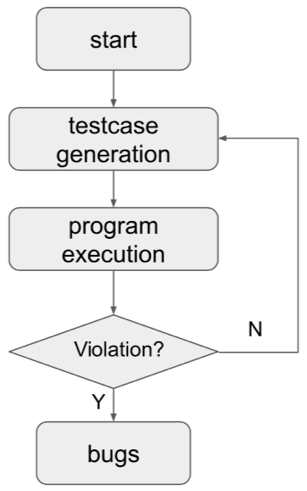
\includegraphics[width=0.5\linewidth]{images/fuzz_stages.png}
  \caption[Fuzzing Stages]{Fuzzing Stages}
  \label{fig:fuzz_stages}
\end{figure}


The main process of the traditional fuzzing process has four main stages, that can be summarized in this way(Figure \ref{fig:fuzz_stages}):
\begin{itemize}
  \item Test case generation stage
  \item Test case running stage
  \item Program execution stage monitoring
  \item Analysis of exceptions
  \end{itemize}


After a bunch of program inputs have been generated (called from here test case), these so generated inputs have to match the requirements of tested program as much as possible. 
Inputs can be of various type, e.g. different file formats, network communication data, executable binaries and so forth.
In state-of-art- fuzzers are used essentially two kind of generators and they are the generation based and mutation based .

Test cases are given to target programs after they have been generated in the previous phase, than fuzzers automatically start and finish the target program process and drive the test cases handling process of target programs. 
Before the execution itself, analysts are able to configure the way the target programs start and finish, and also predefine which parameters and environment variables have to be used. 
In a normal execution, the fuzzing process should stops at a predefined timeout, program execution hangs or crashes. While running, fuzzer monitor the execution state during the execution of the program, seeking for exception and/or crashes.
When some violation is captured by the fuzzers store it in the correspondent test case for latter replay and analysis.
In the subsequent analysis stage, the analyst could try to determine the location and also the root cause of the violations collected. This job can be exploited by means of debuggers like GDB or similar.

\begin{itemize}
  \item \textbf{\textit{Generation Based}}: this kind of fuzzers the knowledge of program input is strictly required, along with a configuration file that basically offer the guide lines to generates test cases.
  \item \textbf{\textit{Mutation Based}}: requires a set of valid initial inputs and test cases are generated throughout the mutation of initial input and test cases generated during the first fuzzing process.
\end{itemize}

\subsection{Types of Fuzzers}
Another important aspect to consider is surely the type of fuzzers that exist. As said above we have generation based and mutation based, but depending on the program source code and the degree of program 
analysis, fuzzers can be also divided and classified in white, grey and black box.
White box are assumed to have all access to the source code and a lot of additional information can be gathered during the analysis on source code and also how test cases have affected the program running state. 
Black box perform fuzzing test without any knowledge of source code while gray one also does not have source code awareness but the information are collected essentially from program analysis.
Another classification is direct fuzzing and coverage-based fuzzing. The goal of a direct fuzzer is to generate test cases that can cover the target code and the target paths of a program and expect a faster test on programs; while a coverage-based fuzzers
try to generate as much code of programs as possible and so expect a more thorough test along with a bunch of bugs discovery. Still, both of them have as a problem, or better as a key challenge, how to extract information of exectuted paths.
The last classification is dumb or smart fuzzer according to wether there is a feedback between the monitoring of a program execution state and test case generation. 

\subsection{Key Challenges in Fuzzing}
There are several challenges that todays fuzzer need to face and solve:
\begin{itemize}
\item mutate seed input
\item low code coverage
\item passing the validation
\end{itemize}

The first one is generically solved by using mutation based generation, but in this case the questions still
arise. Where to mutate and how to do so? Exploiting only mutation on a few key points could affect the the control flow of the program, and how to locate this key "hot-spots" in test cases has a more than fairly importance.
The way how fuzzers mutate has an impacting importance, and so, for what concern blind mutation, it could end up in a serious waste of testing resource while a more conscious mutation strategy could increase and improve the effeciency
of testing significantly. In conclusion, by answering this questions is possible to cover more programs paths and is easier to trigger bugs.
For what concern the second challenge, the work done till now has proved that better coverage results in a higher probability of finding bugs. Despite of that, 
most test cases only cover the same few paths, while most of the code could not be reached and fairly analyzed. So from this we can understand that
it's not a so sensible choice to achieve high coverage only exploiting a large amount of test cases generation and use them as testing resources.
In order to solve this problem, coverage-based fuzzers try to address this problem with the help of some program analysis technique, like code instrumentation. Actually,
this kind of technique is used by AFL and will be discussed further on. 
The last challenge is about validation. Programs, generally, validate inputs before parsing and handling, and the validation works as a sort of guard of programs used to protect program against invalid input and damage that can be caused by malicious constructed
inputs. For example invalid test cases are always discarded or simply ignored.


\subsection{Coverage-Based Fuzzing - AFL}

This kind of strategy is the mostly spread and used by stat-of-the-art fuzzers and has been proved to be one the more effective and efficient.
The fuzzers try to travers as many as running state of the program as possible. Using this such of scheme is still possible to have a loss of information and certain degree of uncertainty.
AFL is one of the kind of fuzzers that exploit this scheme of working.
In the program analysis, the program itself is composed by basic block, that are basically code snippets with a single entry and a single exit point.
The instructions will be sequentially executed and executed only once. In code coverage measuring, state-of-art methods take basic block as the best achievable granularity. That is because of the fact
that basic block is the smallest coherent units in a program execution, measuring function would end up in an information loss or redundancy problem, and finally basic block information can be easily gathered
through code instrumentation. Nowadays, the two basic measurement choices based on basic block are either simply counting the executed one or counting the actual transition performed. In the latest method, what is happen
is that the program is seen and interpreted as a graph, where vertices are used to represent basic block while the edges turn to be transitions between basic block. In this way not only basic blocks are recorded, even edges.
This lead to a better coverage that could not be achieved with a simple basic block recording.
AFL is the first to introduce the edge measurement method into coverage-based fuzzing. Since AFL has been used to perform security analysis in this thesis work, here we show how coverage-based fuzzers
gain coverage information during the fuzzing process. AFL gains the coverage information via lightweight program instrumentation. 
Depending on the source code, AFL provides two instrumentation mode, the compile-in instrumentation and the external one. In the first one, AFL provides
both gcc and llvm mode, which will instrument code snippet when binary code is generated. While in the external mode, basically the qemu mode provided by AFL,
it will instrument code snippet when basic block is translated to TGC block. An example of how the instrumentation of the code is applied is shown in figure \ref{fig:Algo-fuzz}. 

\begin{figure}[tbh]
  \centering
  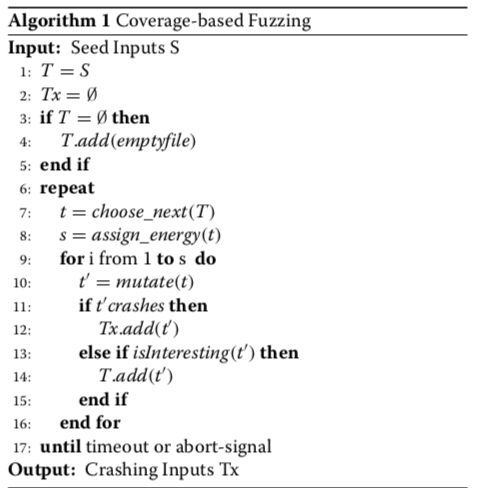
\includegraphics[width=0.7\linewidth]{images/Algo-fuzz.png}
  \caption[Fuzzing Algorithm]{Fuzzing Algorithm}
  \label{fig:Algo-fuzz}
\end{figure}

\subsection{Working process}

The algorithm showed in figure \ref{fig:fuzz-work}, shows the general working process of a coverage-based fuzzer. The test starts it's execution from an initial given seed inputs, 
nevertheless if no input is provided then the fuzzer is able constructs one itself. 
In the main fuzzing loop, the fuzzer repeatedly chooses an interesting seed for the following mutation and test case generation, then the target program is driven to execute the generated test cases under the monitoring of fuzzer.
The resultant test cases that trigger crashes will be collected, and other interesting ones will be added to the seed pool in order to be analyzed in a second moment. 
For a coverage-based fuzzing, all test cases that are able to reach a new control flow edges are considered to be interesting and yet to be used.
 The main fuzzing loop stops at a pre-configured timeout or an abort signal given by the user itself.
During its execution, fuzzers tend to track the execution in different ways. The execution need to be tracked basically for code coverage and security violations.
 The first one is used in order to pursue a meticulous program state execution, while the
second one is used in order to have a better way to trigger and find bugs.

  \begin{figure}[tbh]
    \centering
    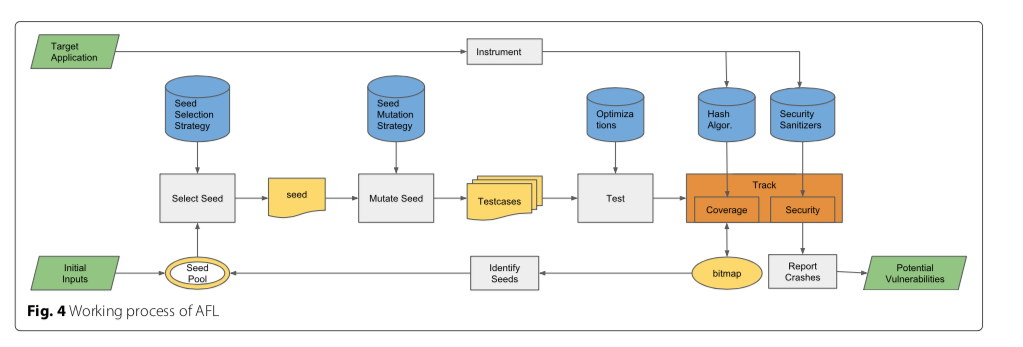
\includegraphics[width=1.0\linewidth]{images/fuzz-work.png}
    \caption[Fuzzing Working Process]{Fuzzing Working Process}
    \label{fig:fuzz-work}
  \end{figure}
  


It's also useful to show how an AFL process works.
The target application is instrumented before execution for the coverage collection, and this instrumentation can be done either compile time or as external, with gcc/llvm mode and qemu mode.
After a seed has been provided to AFL, in the main fuzzing loop, the fuzzer chooses a favorite seed from its pool according to the seed selection strategy,
and usually the smallest and fastest are preferred and so picked up. After that seed files are mutated according to the mutation strategy, and a bunch of test cases are generated.
As last step test cases are executed and the execution is under tracking. Obviously, coverage information is collected in oder to determine which are the interesting test cases (for example the ones that reach new control flow edges), 
in order to add them to seed pool and exploits them for the next round of execution.
%%%%%%%%%%



\subsection{Fuzzing of protocols}
Fuzzing technique has been used to detect several vulnerabilities on different application since it was invented. 
According to the different characteristics of the target application, it's possible to use different fuzzers tha can apply a certain strategy to face different problem.
Since in this work fuzzing is intended to be used against a protocol, it's useful to mark how can be done in this context.
In the recent past, lots of local application have been transformed into network service in a B/S mode. In this configuration, services are deployed on network and client applications can communicate with those exploiting network protocols.
For this reason, security testing on network protocols become more and more crucial and source of concern. Security flaws in protocols could be much worse than a local applications flaws, in fact they can result in serious damages, like DoS attack, information leakage, defacement and so forth.
Several challenges are bond to fuzzing protocols, first one is that services may define their own communication protocols, which are difficult to determine protocol standards. Plus, even for documented one is still hard to follow specification such a RFC document.
By the way, exploiting AFL, we're going to try exploit the flaws found in the \fwh protocol. \cite{fzn}



%%%%%%%%%%
\section{American Fuzzy Lop} %%add historical background, images

As mainly discussed above, fuzzing is one of the most powerful and proven strategies for identifying
security issues in real-world software; it is responsible for the vast majority of remote code execution and privilege escalation bugs found to date in security-critical software.



\subsection{Approach to the problem}
American Fuzzy Lop is a \textbf{brute-force Fuzzer} coupled with an exceedingly simple but rock-solid instrumentation-guided genetic algorithm. 
It uses a modified form of edge coverage to effortlessly pick up subtle, local-scale changes to program control flow.
The algorithm basically works in 6 steps, that are the following:
\begin{enumerate}
  \item Load user-supplied initial test cases into the queue,
  \item Take next input file from the queue,
  \item Attempt to trim the test case to the smallest size that doesn't alter the measured behaviour of the program,
  \item Repeatedly mutate the file using a balanced and well-researched variety of traditional fuzzing strategies,
  \item If any of the generated mutations resulted in a new state transition recorded by the instrumentation, add mutated output as a new entry in the queue.
  \item Go to 2.
\end{enumerate}
  
After test cases have been discovered some of them can be pulled out from newer ones.
As result of the process, the tool is able to create a small self-contained corpus of interesting test cases.
These are very useful in order to seed other.

\subsection{Design goal of AFL-Fuzz}

\begin{description}
    \item[\textbf{Speed}]: afl-fuzz is meant to le you fuzz most of the given targets at approximately their native speed. On top of this, the tool leverages instrumentation
    to reduce the amount of work essentially in two ways, \ie skipping non-functional but non-trimmable regions of the input file or by systematically trimming the corpus 
    \item[\textbf{Rock-solid reliability}]: most of the approach used today based on symbolic execution or similar are unreliable with real world targets, whilst afl-fuzz is
    designed to be rock solid. In fact it is designed to be just a very good traditional fuzzer with a wide range of interesting and useful strategies to go by. 
    \item[\textbf{Simplicity}]: AFL is designed to allows a better understanding of the testing framework even though there is not a complete knowledge of the tool itself.
    Essentially the three knobs you can play with are the output file, the memory limit, and the ability to override the default timeout. All the other settings are supposed to be
    work fine already. When this not apply, warning message are showed to the tester outlining the possible causes and workarounds.
    \item[\textbf{Chainability}]: in order to avoid the creation of custom in-process fuzzers or exploit a massive CPU power again targets that are resource-hungry, AFL tries to
    elude ingeniously this problem by allowing testers to use more lightweight targets in a way to create small corpora of test cases that can be fed into a manual testing or a UI harness.
\end{description}


  
%%%%%%%%%%

\section{\fwh principles} %%UPDATE

Most of the Wi-Fi network that are used today are protected and secured by the WPA2, aka Wi-Fi Protected Access 2.
Even the public hotspots that are wide spread around the world, are running under the WPA2 protocol even though,
authentication is not performed for obvious reason but the encryption should be used instead. Such encrypted networks are so based on the Wi-Fi handshake that is able 
to securely negotiate a fresh pairwise key and exploit this key to ensure that the normal traffic exchange across the network is encrypted.
An essential point of the  work is for sure understand where the \fwh is collocated and how it works during the establishment of secure connection
between a generic client and a generic server.

\subsection{Historical Background}
At his creation, the 802.11 original standard supported a basic security protocol called WEP (Wired Equivalent Privacy), but unfortunately it was designed in a such way that a lot flaws
were present and today is considered completely broken. For those reason the IEEE came up with two solution: a long-term one and short-term one. 
The long-term solution is called (AES-)CCMP, that basically uses an AES in counter mode for confidentiality and CBC-MAC for authenticity. The problem was that most part of the vendors
implemented the cryptographic primitives of WEP in hardware and as a result an incompatibility issue arise and in fact older devices were unable to support CCMP.
In order to solve this problem the short-term solution was designed and it was called (WPA-)TKIP protocol. Basically it's very similar to WEP but it is based on RC4 cipher and this means that
the old devices can support TKIP using only firmware update.
Once the protocol 802.11i was standardized, the WPA2 certification program started, requiring that a device had supporting CCMP and still able to retro-compatibility with the TKIP.

%%%
\subsection{Functioning}
%%TODO: Is better to explain the 4-way in a more precise way or in a general one?
There are 5 different stages that regulates the functioning of the \fwh protocol.
\begin{description}
  

\item [Stage 1: \textit{Network Discovery}]

Networks can be discovered essentially in two ways: passively listening for a beacons, or by actively sending a probe request. When the Access Point (AP) receives those kind of request, it will reply 
to the sender with a probe response. In both cases, the response contains the name and the capabilities of the network, and along with those two, the RSNE will be send.
This will contain several useful element such as contains the supported pairwise cipher suites of the network, the group cipher suite being used, and the security capabilities of the AP.
After the client has found the a valuable network to connect to, the handshake process can start and the connection can be established.
During this phase the client will be known as the "supplicant", while the access point will be called "authenticator".

\item[Stage 2: \textit{Authentication and Association}]

Here the supplicant will start authenticating itself with the authenticator and vice versa, and after this action has been completed the supplicant will continue by associating with the network.
There are four authentication methods defined in 802.11i standard but here we will consider just one of them: the Open System authentication, that allows any supplicant to successfully authenticate.
Once the supplicant has successfully authenticated itself, the association will be done by sending a request to the AP informing it about the features supported. It's important to notice that at this level,
pairwise and group chiper suite are chosen and so that have to been used by the participants. 

\item[Stage 3: \textit{802.1x Authentication}]

This stage is optional and it can be skipped in this work.

\item[Stage 4: \textit{4-Way Handshake}] 

In this stage the formal \fwh is performed in order to provide mutual authentication based on the Pairwise Master Key (PMK), that provides detection function on possible downgrade attack and negotiates a fresh session key called Pairwise Transient Key (PTK).
The PTK is derived from the Authenticator Nonce, Supplicant Nonce, and the Mac address of both supplicant and authenticator. The \fwh generally provides also a Group Temporal Key from the authenticator to the supplicant. Figure \ref{fig:eapol-frame} shows how an Eapol frame is structured.

\begin{description}
  \item[Message 1]: sent by the authenticator and containing randomly generated ANonce of the authenticator itself. Here the two info flags need to be set and they are Pairwise and Ack, represented by label Msg1. It's important
  to notice that at this level there no protection by a MIC (Message Integrity Check), hence for an attacker could be possible to forge this kind of message.
  Once the supplicant has received the message and is aware of the ANonce, it is possible for it to compute and derive the PTK.

  \item[Message 2]: contains the random SNonce of supplicant, and is protected by a MIC. In this message the key info flags to set are Pairwise and MIC, represented by label Msg2. Here it's important to say that in the Key Data Field of the EAPOL message is stored
  the RSNE element, that contains the cipher suite chosen by the supplicant in the association request sent before. Once the authenticator has received this message, is able to calculate the PTK, verify the MIC and check if any miss-match occurs 
  between the old RSNE and the fresh one that has been received. If any discrepancy occurs, the protocol is aborted instantly.

  \item[Message 3]: sent from the authenticator in response to the supplicant, it contains again the ANonce and secure by the MIC as well. The required key info flag here are Pairwise, MIC and Secure (labelled in Msg3), while the Key Data field will contain the supported 
  cipher for the AP. When the supplicant receives this message, ad done previously by the authenticator, the RSNE is checked with the one received when the protocol takes place for the first time, and if the the two RSNE
  differ then a downgrade attack has been detected and the handshake aborted.

  \item[Message 4]: this is the last message and is sent by the supplicant in order to inform the authenticator that the handshake has been completed in correct way. As the previous message, even this one is protected
  by a MIC and the key info flags are Pairwise, MIC and Secure labelled as Msg4. Finally, once the authenticator has successfully received the message 4, encrypted data frames can be transmitted.
\end{description}

\begin{figure}[tbh]
  \centering
  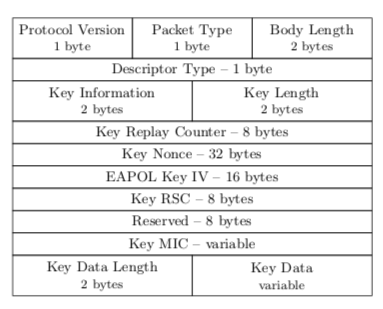
\includegraphics[width=0.8\linewidth]{images/eapol-frame.png}
  \caption[Layout of Eapol-Key frame]{Layout of Eapol-Key frame}
  \label{fig:eapol-frame}
\end{figure}


\item[Stage 5: \textit{Group Key Handshake}]

This last stage is required when a WPA1 is used to transport the group key to the supplicant, and it used to protect from broadcast and multicast traffic. 
The procedure is also used  to periodically renew the group key. The figure \ref{fig:mess-ex} shows the steps that regulate the \fwh during the connection establishment.\cite{asc}

\begin{figure}[tbh]
  \centering
  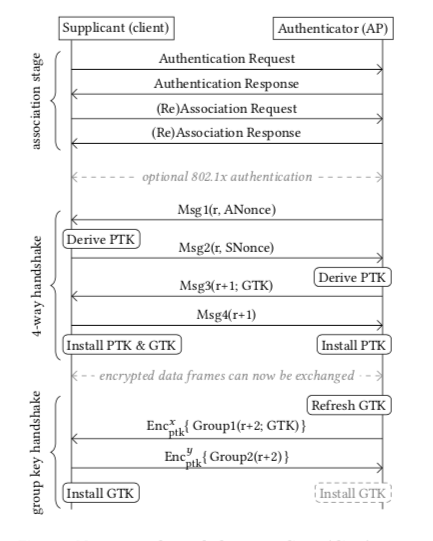
\includegraphics[width=0.8\linewidth]{images/mess-ex.png}
  \caption[Message exchange in \fwh]{Messages exchanged when a supplicant connects to an authenticator.}
  \label{fig:mess-ex}
\end{figure}



\end{description}

\section{The KRACK attack}

After a brief overview on how the \fwh protocol works, now it's important to understand in which way is possible to attack and exploit its vulnerabilities.
The Key Reinstallation Attack (\krack) abuses of a protocol to reinstall an already in-use key 
by resetting the nonces and/or the replay counters associated to it. In its 14 years lifetime, the \fwh has been thought to be secure due to the fact that no weaknesses were discovered during this time and plus it was proven to be secure.
But in this kind of attack, the adversary can trick a victim in reinstalling an already in-use key without be conscious of it.

Nowadays all the Wi-Fi networks that are used, have a as the WPA2 protection as defense mechanism against possible attack. This kind of technology relies obviously on the \fwh defined in the standard 802.11i.
As said previously the \fwh provides mutual authentication and also a session key agreement for the authenticator and the supplicant. This can be achieved thanks to the (AES-)CCMP, data-confidentiality and integrity, and since its introduction 
in the 2003 no breaches in the protocol have been found, apart from the weaknesses encountered by using TKPI (that was uniquely a short term solution).
The idea behind the attack actually is more trivial that one can imagine, and can be sketched in the following way. Let's consider a client joins a network, the \fwh is executed in order to negotiate a fresh session key. This key is usually installed after message 3 has been received, and it will be used
to encrypt data frames using a confidentiality protocol. At this point it's important to notice the fact that messages can be lost or even dropped, so the AP, in this case, is in charge to retransmit the message if do not receive a proper response as acknowledgment from the supplicant. Since this mechanism is easily 
understandable that message 3 can be received multiple times, and each time it will reinstall the same session key, but resetting the nonce and the receive replay counter used by the data-confidentiality protocol.
Now what an attacker can do is forcing these nonce resets by collecting and replaying transmission of message 3, and this manner the data-confidentiality protocol can be exploited and attacked. For example, the packets sending through the channel are subject to replay, decryption and/or forging.
The same technique is also used to attack the group key, PeerKey and the FBSS transition handshake.
The attack above described turned out to be devastating against version 2.4 and higher of "wap-supplicant", that is one the Wi-Fi most commonly used in Linux system. Since Android uses a modified version of the "wpa\_supplicant", all the Android version from the 6.0 to the newer one are effected.

\subsection{Supplicant state machine}

In order to understand how the attack is mounted is necessary to have a look at the supplicant state machine and spot the weaknesses of the protocol itself.
The 802.11i amendment does not contain a formal state machine that explain how the supplicant has to be implemented, it just provide a pseudo-code that describe
how, but not when, a certain message should be processed and handled. In one of it's extension, precisely the 802.11r, the \fwh protocol come along with 
a detailed state machine of the supplicant (show in figure \ref{fig:sup-sm}).
When a connection to a network took place and the \fwh starts, the supplicant transitions to a PTK-INIT state. In this way it initializes the PMK, and 
after receiving message 1 it transitions to the PTK-START stage. This could occurs in two situation: when connecting to a network for the very first time or when the
session key is being refreshed after an already terminated \fwh. As soon as the supplicant enter in the PTK-START stage generates a random SNonce, compute the 
Temporary PTK and then sends its nonce to the authenticator by using message 2. At this point the authenticator will reply with message 3, which will be accepted by the supplicant
only if the MIC and the reply counter are valid. If its the case, the supplicant passes to the PTK-NEGOTIATING state, in which it marks the TPTK as valid and sends message 4 as reply to 
the authenticator. Then it moves to the PTK-DONE state, where the PTK and GTK are installed for usage by the data-confidentiality protocol. At the end of this process
the 802.1X port it's opened and the supplicant is able to receive and send normal data frames. Here it's possible to notice that either message 1 or 3 can be retransmitted 
when message 2 or 4 are not received by the authenticator. These retransmissions are possible thanks to the EAPOL replay counter.


\begin{figure}[tbh]
  \centering
  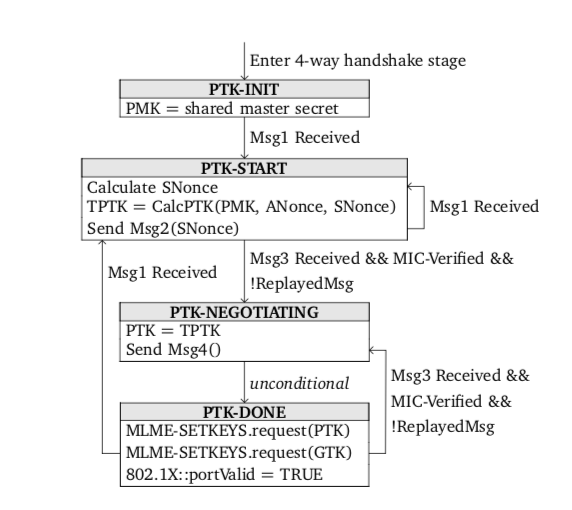
\includegraphics[width=0.8\linewidth]{images/sup-sm.png}
  \caption[Supplicant State Machine]{Supplicant State Machine}
  \label{fig:sup-sm}
\end{figure}

\subsection{Key Reinstallation Attack}

After taking into account the functioning of the state machine, it's now possible dive into the attack itself. Since the supplicant accepts retransmissions of message 3, even
when it is in the PTK-DONE stage, it's possible to force the reinstallation of th PTK. Specifically, the attacker first establish a man-in-the-middle (MitM) position between the 
supplicant and the authenticator, and then by exploiting his position can trigger the retransmissions of message 3 by preventing message 4 from correctly arriving to the authenticator
itself. As a consequences, it will retransmit message 3 and the supplicant will forced to reinstall an already-in-use PTK. In turn, this will reset the transmit nonce and the receive replay
counter that is currently used by data-confidentiality protocol. Notice here that depending on which protocol is used, the attacker is allowed to replay, decrypt and/or forge packets freely.

\subsection{Plaintext Retransmission of message 3}

In the scenario presented above, if we consider the victim still accepting the plaintext retransmissions of message 3 after it has already installed the session key, it's easy to understand how 
the key reinstallation attack is straightforward. In the initial step, the attacker can use a channel-based MitM attack in which way he can manipulate as he desire the handshake messages. Soon after
this operation is been set, he can prevent message 4 from arriving at the authenticator, showed in figure \ref{fig:mitm}.
As soon as message 4 has been sent the victim will install both PTK and GTK, and at this point also the 802.1x port will be open. This will infer that from now on normal data frames can be transmitted.
Then, in the third stage of the attack, the authenticator will retransmit message 3 because it didn't receive message 4 since it has been intercepted by the attacker. At this point the latter forwards the
retransmitted message 3 to the victim inducing the victim to reinstall the PTK and GTK. As result of this action both replay counter and nonce used by data-confidentiality protocol are reset.
It's important to underline here that the attacker cannot replay an old message 3 due to the fact that its EAPOL replay counter is no longer fresh and so it would be refused. Let's omit temporary the stage 4
and skip forward. In the end, when the victim retransmit its next data frame, the data-confidentiality protocol will reuse nonces. The attacker have the faculty of manages both the forwarding time between messages
and the amount of nonces that can be reused as well. Moreover, the client could be de-authenticated by the attacker, after which it will reconnect to the network performing a new \fwh.
In figure \ref{fig:mitm}, is possible to notice that even though no attack has been mounted by third party, the \krack attack can happen spontaneously if message 4 is lost due to background noise.
Basically would happen when the client that accepts plaintext retransmissions of message 3 may already be reusing nonces without no one forcing it to do so. 

Go back to the stage 4, that is the one in charge of completing the handshake at the authenticator side. Since the victim has already installed the PTK, the message is now encrypted making this step no so trivial; plus 
the the authenticator will reject this message for due to the fact that its PTK is not installed yet. In principle this should happen but carefully analyzing the 802.11 standard has been noticed that the authenticator may actually
accept \textit{any} replay counter used in the \fwh previously. Basically some APs accept replay counters that were used in a message to the client, but were not yet used in a reply from the client. In that way those APs will accept
the older unencrypted message 4 which has a replay counter r + 1, as showed in figure \ref{fig:mitm}. As result of this action, the PTK will be installed and the AP will start sending encrypted unicast data frames to the client.
As said before, tha attacked has been confirmed works against \textit{wpa\_supplicant} that is used by Linux and Android.\cite{krk}


\begin{figure}[tbh]
  \centering
  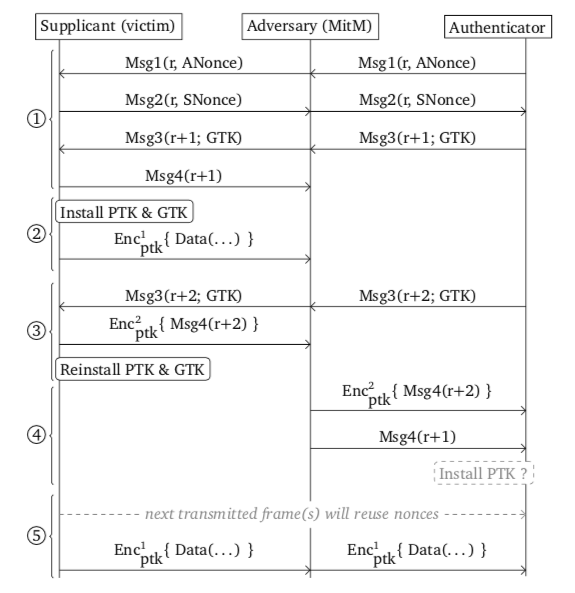
\includegraphics[width=0.8\linewidth]{images/mitm.png}
  \caption[Key Reinstallation attack]{Key Reinstallation attack when the victim still accept message 3}
  \label{fig:mitm}
\end{figure}



%%%%%%%%%%%%%%%%%%

\section{iNet Wireless Daemon}
For what concern IWD the only information that I've been able to recover for the moment are these following.

iNet Wireless Daemon (aka iwd) project aims to provide a comprehensive Wi-Fi connectivity solution for Linux based devices, and
it has been written by Intel basically with aim of replacing WPA Supplicant.
The core goal of the project is to optimize resource utilization: storage, runtime memory and link-time costs. 
This is accomplished by not depending on any external libraries and utilizes features provided by the Linux Kernel to the maximum extent possible. 
The result is a self-contained environment that only depends on the Linux Kernel and the runtime C library.
Definition from \url{https://iwd.wiki.kernel.org}{iwd getting started}.


\section{Work done}
A brief description of the practical work that I've done in the passed weeks and my goal for the next weeks.

\subsection{AFL-tutorial}

In the passed weeks I have completed the remaining challenge of the tutorial, that actually took me more time than expected, but anyway useful to better understand how AFL behaves in different 
cases and context. Plus I've attended an interesting lecture given by my supervisor that was about IoT, but he covered fuzzing and low level security as well. We also had a pratical session during we have 
exploited some toy code with and without AFL. 

\subsection{IWD} 
Dealing with this tools presented some issues due to the fact that I'm using Linux Ubuntu on a VM, and apparently
there a no Wireless interface in the current version of Parallels or VirtualBox for Linux Ubuntu. This problem, that initially was intended to be solved
by using an USB NIC, has turned out to be a dead end. There were several incompatibility issues that we're not able to overcome and so we decided to use another approach.
In order to create a test wifi network, we use "hostapd" as server and yet iwd as client. Hostapd (host access point daemon) is a user space daemon software enabling a network interface card to act as an access point and authentication server. 
To do so it has been necessary to run both iwd AP and client as virtual hardware. After both AP and client have been started it is possible to acually establish a connection, and 
using Wireshark I tested the proper exchange of message between the two participants involved. 

\subsection{Goals}
Currently I'm trying to get an initial approach to the real work, and specifically, my goal is to analyze the "test-eapol.c" source code that is used by iwd to test the actual 
functioning of the \fwh. I'm planning to understand the source code and is it implemented and I'll try to figure it how to modify it. My current idea is to create a sort of harness code in the function that deal with 
the sending of message no.3 of the \fwh. I'm going to analyze the first packet contents in order to fuzz it by feeding with random data.
After this initial step, I should come up with a solution for fuzzing packet no.2 and so forth.
In my idea this analysis could be done "off-line" since the testing are done statically, further on I think that an "online" analysis could be performed.









\chapter{N/A}


\chapter{Design - N/A}

Discutere in questo capitolo come � stata progettata la soluzione al problema trattato nella tesi, indicando anche se sono stati valutati vari possibili approcci o soluzioni pre-esistenti e giustificando le proprie scelte. Descrivere quindi la soluzione vera e propria.

Nel caso sia stato sviluppato del software non triviale, � buona norma dedicargli tre sezioni:
\begin{itemize}
\item architettura dell'applicazione (interazioni con gli utenti e con altri sistemi, moduli logici, flussi dati interni ed esterni);
\item manuale dello sviluppatore (descrizione dei moduli, degli algoritmi, delle interfacce e delle strutture dati);
\item manuale utente (come installare ed usare il programma, interfacce, comandi, dati in input ed in output).
\end{itemize}
Nel caso di software molto voluminoso, queste tre sezioni possono diventare tre capitoli separati.

\chapter{Results- N/A}

Inserire in questo capitolo i risultati conseguiti, cercando di analizzarli -- se possibile -- in modo quantitativo.


\chapter{Final Conclusions - N/A}

Qui si inseriscono brevi conclusioni sul lavoro svolto, senza ripetere inutilmente il sommario.

Si possono evidenziare i punti di forza e quelli di debolezza, nonch� i possibili sviluppi futuri o attivit� da svolgere per migliorare i risultati.

% bibliografia scritta "a mano"
% !TEX encoding = IsoLatin

% La bibliografia, da inserirsi solo se ci sono state citazioni.
% In questo caso ricordarsi che bisogna sempre elaborare due volte il file .TEX
% perch� la prima volta viene generata la bibliografia mentre la seconda volta viene inclusa

% NOTA: citare il DOI non � obbligatorio ma MOLTO desiderabile

\begin{thebibliography}{9} % se ci sono meno di 10 citazioni
%\begin{thebibliography}{99} % se ci sono da 10 a 99 citazioni
%\begin{thebibliography}{999} % se ci sono da 100 a 999 citazioni

%%ASIACS PAPER
%citation on paper
\bibitem{asc}
%author
Vanhoef, M and Schepers, D and Piessens, F,
%title
``Discovering logical vulnerabilities in the Wi-Fi handshake using model-based testing'',
% name of the journa�
ASIA CCS 2017 - Proceedings of the 2017 ACM Asia Conference on Computer and Communications Security,
% %volume and number of the journal (may not be present)
%Vol.\ 1,
% year and month of publishing
2017,
% page of the article
pp.\ 360-371,
% DOI
\doi{110.1145/3052973}


\bibitem{krk}
% nome del progetto
OPCDE, Dubai, 7 April 2018, Vanhoef
 % URI della pagina web
\url{https://papers.mathyvanhoef.com/opcde2018-slides.pdf}



%%FUZZING PAPER
\bibitem{fzn}
Li, Jun and Zhao, Bodong and Zhang, Chao,
``Fuzzing: a survey'',
Cybersecurity,
Vol.\ 1,
2018,
pp.\ 1-13,
\doi{10.1186/s42400-018-0002-y}


\bibitem{img}
% nome del progetto
Fuzzing image
 % URI della pagina web
\url{https://medium.com/@dieswaytoofast/fuzzing-and-deep-learning-5aae84c20303}



\end{thebibliography}


% se la bibliografia � stata scritta (usando Bibtex) nel file biblio.bib allora commentare la riga precedente e scommentare le due righe seguenti
%\bibliographystyle{torsec}
%\bibliography{biblio}


\end{document}
